\documentclass[twocolumn,10pt]{article}
\usepackage{geometry}
\usepackage{amsmath}
%\usepackage[cmintegrals]{newtxmath}
%\usepackage{bm} % optional
\usepackage{cite}
%\usepackage[dvipdfmx]{graphicx}
\usepackage{graphicx}
\usepackage{color}
\usepackage{lscape}
\usepackage{url}
\usepackage{amssymb}
\usepackage{bm}
\usepackage{comment}
\usepackage{fancybox}
\geometry{left=20mm,right=20mm,top=10mm,bottom=10mm}
\thisfancyput(13.0cm,1.0cm){\textcolor{red}
 {\doublebox{\large{\bf{Do Not Disclose}}}}}
\begin{document}
\title{Siamese Network for Classification with \\ Optimization of ROC-AUC}
\author{M181021 Hideki Oki \\ Department of Information Engineering}
\date{\empty}
\maketitle
\begin{abstract}
The original form of Support Vector Machine (SVM) was first invented by V. Vapnik et al. \cite{Vapnik1963} in 1963 and the current standard from of soft-margin SVM was proposed by C. Cortes et al. \cite{SVM1995} in 1995.
The SVM is defined to solve the binary classification problem, the idea of SVM is extended to other tasks.
For example, RankSVM was proposed by R. Herbrich et al. \cite{RankSVM} for learning to rank. 
RankSVM is the pairwise learning model and is currently used most frequently as a baseline in the field of rank learning such as information retrieval.
O. Chapelle et al. \cite{ROCAUC} show that RankSVM can optimize ROC-AUC for binary classification.
Meanwhile, a deep neural network model such as deep Convolutional Neural Network (CNN) has been widely used in the field of pattern recognition since deep CNN proposed by Krizhevsky et al. \cite{Krizhevsky2012} won the ILSVRC 2012 with higher recognition accuracy than the conventional methods.
To enable pairwise learning by deep neural networks, 
models such as Siamese Neural Network \cite{Bromely1993,Chopra2005,Hadsell2006} have been developed and used for rank learning.
And,objective function of Siamese Network is the same function as RankSVM.
This means that Siamese Network can also optimize ROC-AUC for binary classification.
To the best of our knowledge, we can not find the research in which Siamese Network is used for optimizing ROC-AUC for the classification tasks.
In this paper we experimentally confirm whether ROC-AUC can be optimized by Siamese Network for rank learning.
For the purpose of verification, we compare the ROC-AUC score in binary classification of the standard CNN model which trained by sigmoid crossentropy loss with the model which was trained by using Siamese Network for rank learning.
\end{abstract}
\section{Introduction}
The original form of Support Vector Machine (SVM) was first invented by V. Vapnik et al. \cite{Vapnik1963} in 1963 and the current standard from of soft-margin SVM was proposed by C. Cortes et al. \cite{SVM1995} in 1995.
It is known that the the standard SVM is formulated as convex optimization problem and has unique global optima.
Also, we can easily extend the linear SVM to the nonlinear SVM by introducing kernel learning.
%Since SVM does not converge in local solution and generalization performance is high, it has been widely used in pattern recognition.
The SVM is defined to solve the binary classification problem, the idea of SVM is extended to other tasks.
For example, RankSVM was proposed by R. Herbrich et al. \cite{RankSVM} for learning to rank. 
RankSVM maximizes the margin between samples that are highly relevant to the query and those that are less relevant to the query whereas 
the standard SVM maximizes the margin between classification boundaries and training samples.
RankSVM is the pairwise learning model and is currently used most frequently as a baseline in the field of rank learning such as information retrieval.
O. Chapelle et al. \cite{ROCAUC} show that RankSVM can optimize ROC-AUC for binary classification.
This is realized by optimizing the parameters of RankSVM as maximizing the margin between positive class and negative class. 
However, it is difficult to estimate the class from the output value only by maximizing the margin of the positive class and the negative class.
Therefore, O. Chapelle et al. manually adjust the output value at the learning stage so that the output value for the positive class is larger than the output value for the negative class. \par
Meanwhile, a deep neural network model such as deep Convolutional Neural Network (CNN) has been widely used in the field of pattern recognition since deep CNN proposed by Krizhevsky et al. \cite{Krizhevsky2012} won the ILSVRC 2012 with higher recognition accuracy than the conventional methods.
To enable pairwise learning by deep neural networks, 
models such as Siamese Neural Network \cite{Bromely1993,Chopra2005,Hadsell2006} have been developed and used for rank learning.
Siamese Neural Network maximizes the distance between the sample that is highly relevant to the query and the sample that is less relevant to the query, and minimize the distance between samples that are highly relevant to the query or between those that are less relevant to the query.
This objective function of Siamese Network is the same function as RankSVM.
This means that Siamese Network can also optimize ROC-AUC for binary classification.
\thispagestyle{empty}

To the best of our knowledge, we can not find the research in which Siamese Network is used for optimizing ROC-AUC for the classification tasks.
In this paper we experimentally confirm whether ROC-AUC can be optimized by Siamese Network for rank learning.
For the purpose of verification, we compare the ROC-AUC score in binary classification of the standard CNN model which trained by sigmoid crossentropy loss with the model which was trained by using Siamese Network for rank learning.
In RankSVM, the output value was adjusted manually so that the class can be estimated from the output value.
Instead of manually adjusting the output value of Siamese Network, we decided to divide the learning into two stages.
The first stage, maximizes margin of positive class and negative class by optimizing loss of siamese network.
In the second stage, we make it possible to estimate the class from the output by learning logistic regression model using the feature vector obtained from this Siamese Network to express posterior probability.
By doing this, we think that the value for estimating the class more natural can be obtained from Siamese Network.

Then, the model using Siamese Network for binary classification is extended to multi class classification problems. The ROC-AUC of the proposed model is also compared with the standard deep CNN model for multi-class classification.

\section{Related Works}

\subsection{Deep Convolutional Neural Network}

The deep CNN has been proved to be effective and has been applied many applications such as for image classification\cite{Krizhevsky2012,He2016}, object detection\cite{He2017}, image segmentation\cite{Ronneberger2015} and so on.

The computation within the convolution layers is regarded as a filtering process of the input image as
\begin{align}
f_{p,q}^{(l)}=h(\sum^{convy-1}_{r=0}\sum^{convx-1}_{s=0}w^{(l)}_{r,s}f^{(l-1)}_{p+r, q+s}+b^{(l)}) \; ,
\end{align}
where $w^{(l)}_{r,s}$ is the weight of the neuron indexed as $(r,s)$ in the $l$-th convolution layer and $b^{(l)}$ is the bias of the $l$-th convolution layer. 
The size of the convolution filter is given as $convx \times convy$. The activation function of each neuron is denoted as $h$. 
Usually, pooling layers are added after the convolution layers. The pooling layer performs downsampling for reducing computational costs and enhancing against micro position changes. 
Fully-connected layers like multi layer Perceptron is connected to the convolution layers which is used to construct the classifier. 

\subsection{Siamese Network}
\begin{figure}[ht]
\begin{center}
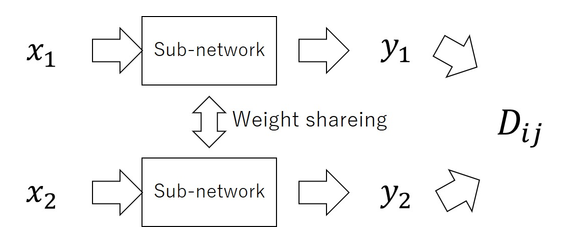
\includegraphics[width=70mm]{figure1.eps}
\caption{Siamese Network}
\label{fig:siamese}
\end{center}
\end{figure}

The Siamese Network \cite{Bromely1993,Chopra2005,Hadsell2006} consists of two identical networks joined at their outputs as shown in Figure \ref{fig:siamese}.
The two networks extract feature vectors from two different samples.
Usually, the weights of the two networks are shared, the objective function of the optimization for training the parameters of the networks is defined by using these extracted feature vectors.
The parameters of the Siamese Network are trained to distinguish between similar and dissimilar pairs of the training samples. 
This network architecture is usually used for metric learning, and a contrastive loss over the metric defined on the trained representation is used as the objective function for the optimization. The objective function is defined as
\begin{align} \label{eq:contrastive}
E&=\frac{1}{2N}\sum_i^N \sum_j^N l_{ij}(D_{ij})^2 \notag \\
&+ (1-l_{ij})max(m-D_{ij}, ~0)^2 \\
D_{ij}&=||{\bm y}_{i}-{\bm y}_{j}||^2_2
\label{eq:dis}
\end{align}
where $m$ is a parameter indicating the distance between clusters and 
$D_{ij}$ represents the distance between the pair of the outputs $\bm{y}_i$ and $\bm{y}_j$ of each network for the sample pair $\bm{x}_i$ and$\bm{x}_j$.
A label $l$ is assigned for each sample pair such that 
label is $l_{ij}=1$ when the pair $i$ and $j$ is similar and label is $l_{ij}=0$ when the pair $i$ and $j$ is dissimilar.
After the training of Siamese Network, the outputs for dissimilar pair will be dissimilar while the outputs for similar pair become similar.


\subsection{Rank SVM}

The RankSVM is a ranking model minimizing margin-based pairwise loss \cite{RankSVM}.
RankSVM was trained to minimize the loss function defined by
\begin{align} \label{eq:RankSVM}
    \frac{1}{2}||{\bm w}||^2+\lambda \sum_{i \in P, j \in N}max(0, 1-{\bm w}^T({\bm x}_i - {\bm x}_j))^2
\end{align}
where $P$ is a set of positive training samples, and $N$ is a set of negative training samples. 
$\lambda$ is a parameter of $\lambda > 0$, ${\bm w}$ is a weight.
And $({\bm x}_i, {\bm x}_j)$ is a pair of training samples given a positive label and a negative label.
As can be seen from equation (\ref{eq:RankSVM}), among the pairs of the positive vector and the negative vector, the loss becomes large when the pair is incorrectly ranked.

O. Chapelle et al. \cite{ROCAUC} proposed a fast optimization method for RankSVM based on the primal Newton method.
Also, O. Chapelle et al. showed that RankSVM can be used for binary classification and can improve area under the ROC curve (AUC) defined as 
%(Equation(\ref{eq:AUC})) as a evaluation criterion.
\begin{align} \label{eq:AUC}
    AUC=\frac{|\{(i,j)| t_i=1, t_j=0, f({\bm x}_i) > f({\bm x}_j)\}|}{|\{i|t_i=1\}| \times |\{j|t_j=0\}|}
\end{align}
where $t_i \in \{1,0\}$ is a label assigned to $i$-th training sample and $|S|$ denotes the number samples in the set $S$.
$f({\bm x}_i)$, $f({\bm x}_j)$ are outputs of RankSVM for samples ${\bm x}_i$, ${\bm x}_j$.
The denominator is the product of the number of positive samples and the number of negative samples and the numerator is the number of pairs that positive and negative samples could be classified correctly.
In order to optimize the loss defined by the equation (\ref{eq:RankSVM}), the ranking of ${\bm x_i}$ and ${\bm x_j}$ must be correct.
That means that the ROC-AUC score should be high. 
This has been introduced as a special case of RankSVM.

\section{Proposed Method}
\thispagestyle{empty}

O. Chappell et al. \cite{ROCAUC} show that RankSVM can be used to construct a binary classifier for optimizing the ROC-AUC.
%RankSVM can learn ranking.
Binary classification is realized by using RankSVM and by maximizing the margin of positive sample and negative sample. 
%Also, the authors show that RankSVM can be used to construct a binary classifier for optimizing the AUC.
%In other words, RankSVM assumes that a positive sample and a negative sample are input as a pair, and it learns their ranking.
Since the Siamese Network for rank learning uses the same loss function with RankSVM,
the Siamese Network also can be used to construct a binary classifier for optimizing the ROC-AUC.
%learn to output the similar feature vectors to the samples in the same class and to output different feature vectors for the samples of different classes.
%And, in addition to ranking positive samples and negative samples, the Siamese Network also learns the relationship between samples of the same class.
%Therefore, in classification, we think that Siamese Network also can optimize AUC like RankSVM. 
In this paper, we propose to use the Siamese Network for rank learning for constructing a binary classifier.
Then the proposed method is extended to multi-class classification problem.


\subsection{Binary Classification}
\thispagestyle{empty}

\begin{figure}[ht]
\begin{center}
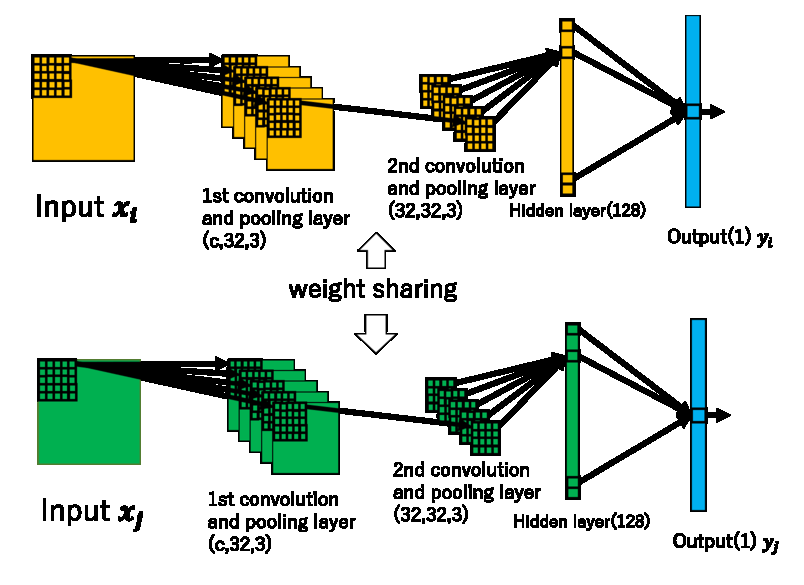
\includegraphics[width=70mm]{figure2.eps}
\caption{Siamese Network for binary classification}
\label{fig:siamese-bi}
\end{center}
\end{figure}

In order to perform binary classification, consider the Siamese Network which classify the positive class and the negative class as shown in Figure \ref{fig:siamese-bi}.
The output of each network $y$ is assumed to be scalar, namely the dimension of the output is $1$.
Similar with the standard Siamese Network, the weights of the two networks are shared.
ReLU is used as an activation function for each convolution layer and hidden layer. 

The objective function of the Siamese Network for binary classification is defined as
\begin{align} \label{eq:siamese-loss}
E&=\frac{1}{2N}\sum_i^N \sum_j^N l_{ij}(D_{ij})^2 \notag \\
&+ (1-l_{ij})max(m-D_{ij}, ~0)^2 \\
D_{ij}&=||y_{i}- y_{j}||^2_2
\label{eq:siamese-dis}
\end{align}
where $m$ is a parameter indicating the distance between clusters and 
$D_{ij}$ is the distance between the pair of the outputs $y_i$ and $y_j$ of each network for the sample pair $\bm{x}_i$ and$\bm{x}_j$.
For the binary classification, the label is defined as $l_{ij}=1$ whenever the pair of inputs ${\bm x_i}$ and ${\bm x_j}$ belongs to the same class and $l_{ij}=0$ whenever the pair of inputs belongs to the different class.

%Since the output is one value, $D_{ij}$ used in the contrastive loss of equation (\ref{eq:contrastive}) is changed from equation 
%(\ref{eq:dis}) as follows.
%\begin{align}
%D_{ij}&=|y_{i}- y_{j}|^2
%\label{eq:binary dis}
%\end{align}
%We assume label $t_{ij}=1$ whenever input ${\bm x_i}$ and ${\bm x_j}$ belong to the same class.
%And, we assume label $t_{ij}=0$ whenever input ${\bm x_i}$ and ${\bm x_j}$ belong to the different class.


The objective function of the Siamese Network depends on the distances between pair of samples and the order of the output of positive class $y_+$ and the output of negative class $y_-$ is not specified.
On the other hand, AUC assumes the order $y_+ > y_-$.
This means that there is a possibility to be inconsistent of the order of the outputs.
To make consistent and to estimate the posterior probability $P(l=1|\bm{x})$, we apply the logistic regression to the output of the trained network $y$. 
%At the time of model evaluation, a positive sample is input to one network and a negative sample is input to the other network, and AUC is calculated from the output result.
%And, the siamese network has no constraints on the area to cluster each class.
The logistic regression model is given by
\begin{align} \label{eq:regression}
    P(l=1|\bm{x}) \approx \hat{y} = \sigma(w y+b)
\end{align}
where $w$ and $b$ is the parameters of the model and $\sigma(\cdot)$ is the sigmoid function.
Usually the log-likelihood of the logistic regression for $N$ training samples is defined by
\begin{align} \label{eq:crossentropy}
    L = \sum_{i=1}^N \{ t_i log(\hat{y}_i) + (1-t_i) log(1-\hat{y}_i) \}
\end{align}
The optimum parameters $w$ and $b$ are obtained by maximizing this log-likelihood.

%$b$ is a bias, and $w$ is updatable weight, the gradient $\frac{\partial E}{\partial w}$ is calculated based on the loss derived from crossentropy loss(Equation (\ref{eq:crossentropy})) and it is updated by MomentumSGD.
%\begin{align} \label{eq:crossentropy}
%E = -\sum_{n}^N t_n log(\hat{y}_n) + (1-t_n) log(1-\hat{y}_n)
%\end{align}
%In the case of crossentropy loss, let the label of positive class be $t_n = 1$ and the label of negative class be $t_n = 0$.
%After 10th epoch, calculate the AUC using each $\hat{y}_n$ obtained.

In the proposed method, Siamese Network is regarded as a feature extractor and the obtained features are classified by logistic regression model.
As can be seen from Equation (\ref{eq:crossentropy}), it is obvious that the output value becomes larger for the positive class.
%Therefore, the above problem is solved. \par

%First, the average $\bar{y}$ of all output values is subtracted from each all output value $y_n$.
%\begin{align} \label{eq:avey}
 %   \acute{y}_n &= y_n - \bar{y}
%\end{align}
%As a result, the average of the output values is set to 0. \par
%Second, since there is a possibility that positive classes are clustered in the negative direction, the following %operation is performed on each output value.
%\begin{eqnarray} \label{eq:ypn}
%\hat{y}_n = \left\{
%\begin{array}{ll}
%-\acute{y}_n & (a < 0) \\
%\acute{y}_n & (otherwise)
%\end{array}
%\right.
%\end{eqnarray} 
%Here, 
%\begin{align} \label{eq:a}
%a = \frac{1}{PN}\sum_{i}^{P}\sum_{n}^{N}y_i-y_n \; .
%\end{align}
%$P$ is the total number of positive samples, and $N$ is the total number of samples.
%As a result of this operation, $\hat{y}_n$ meets the prerequisite of AUC. \par


\subsection{Multi-class Classification}

\begin{figure}[ht]
\begin{center}
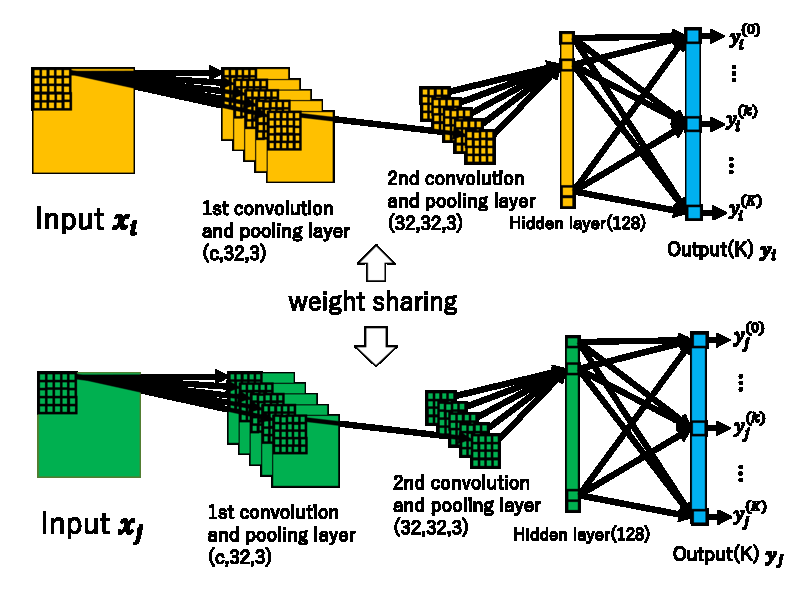
\includegraphics[width=70mm]{figure3.eps}
\caption{Siamese Network for multi-class classification}
\label{fig:siamese-mu}
\end{center}
\end{figure}
We extend the proposed binary classifier to multi-class classification by using one-vs-others approach.
%feature extractor in the binary classification proposed in the previous subsection to the multi-class feature extractor.
Figure \ref{fig:siamese-mu} shows the proposed Siamese Network for multi-class classification.
Similar with the Siamese Network for binary classification, the $K$ features $y^{(1)},y^{(2)},\ldots,y^{(K)}$ for $K$ classes classification are extracted by deep CNN.
%Each convolution layer and fully connected hidden layer are constructed in the same way as in the case of binary classification, and making the number of units of the output layer equal to the number of classes to be classified.

Each unit in the output layer of Siamese Network extracts a feature to classify the corresponding class and the other classes.
The constrastive loss of this network is defined as
%Each unit functions as a feature extractor such as in the case of a specific class and others classification. That is, considering the classification of $K$ classes now, labels are allocated to each unit, and contrastive loss is calculated for the output of each unit as shown in Equation (\ref{eq:multi contrastive}).
\begin{align} \label{eq:multi contrastive}
E_k&=\frac{1}{2N}\sum_i^N \sum_j^N l_{ij}^{(k)}(D^{(k)}_{ij})^2 \notag \\
&+ (1-l_{ij}^{(k)})max(m-D^{(k)}_{ij}, ~0)^2 \\
D^{(k)}_{ij}&=|y^{(k)}_{i}- y^{(k)}_{j}|^2
\end{align}
where $l_{ij}^{(k)}$ is a label to indicate the binary classification of the $k$-th class and the other classes.
The distance $D^{(k)}_{ij}$ is defined as the distance between the pair of outputs $y_i^{(k)}$ and $y_j^{(k)}$ of the $k$-th unit.

The average of $K$ constrastive losses $E_k$  
\begin{align} \label{eq:ave contrastive}
E = \frac{1}{K}\sum_{k}^{K}E_k
\end{align}
is used to obtain the weights of the Siamese Network.
%Then, $k$-th unit of the output layer independently learns features for classifying the $k$-th class and others. \par

To estimate the posterior probability of each class from the features calculated by the Siamese Network, we use the multi-nominal logistic regression.
%Also in the case of multi-class classification, the problem of output described in the previous subsection occurs.
%Therefore, we extend the linear regression model described in the previous subsection for multi-class classification. \par
%In the case of multi-class classification, the number of output dimensions of siamese network is the number of classes to be classified.
The model of the multi-nominal logistic regression for the input vector $\bm{x}$ is given as
%So, the model of Equation (\ref{eq:regression}) is modified as follows.
\begin{align} \label{eq:regression multi}
    \hat{\bm y}_n = S(W\bm{y}_n+\bm{b})
\end{align}
where $W$ and $\bm{b}$ are the coefficient matrix and the bias vector respectively.
%Here, 
%\begin{align} \label{eq:string def}
%{\bm y}_n=\left[
%\begin{array}{c}
%y_n^{(0)} \\ 
%y_n^{(1)} \\
%\vdots \\
%y_n^{(K)}
%\end{array}
%\right], \hspace{0.2cm}
%W =\left[
%\begin{array}{ccc}
%w_{00} & \cdots & w_{0K} \\ 
%\vdots & \ddots & \vdots  \\
%w_{K0} & \cdots & w_{KK} \\
%\end{array}
%\right]
%\end{align} 
%Each element of ${\bm w}$ is an updatable weight and ${\bm b}$ is a bias. 
Also, $S(\cdot)$ is a softmax function.
%In the case of multi class, the label ${\bm t}$ expresses which class a specific sample belongs with one-hot-vector.
Similar with the binary logistic regression, the log-likelihood for the training samples is defined as
\begin{align} \label{eq:multi crossentropy}
L = \sum_n^N {\bm t}_n^Tlog(\hat{\bm y}_n) \; 
\end{align}
where $log(\hat{\bm y}_n)$ is the logarithm of each element of $\hat{\bm y}_n$. 
This is used to obtain the optimum parameters $W$ and $\bm{b}$ of the model.
It is known that this log-likelihood is the same as the cross entropy loss except the sign.
%\par
%As in the previous subsection, the optimum parameters ${\bm w}$ and ${\bm b}$ are obtained by maximizing this log-likelihood. \par


\section{Experiment}
\thispagestyle{empty}

In the experiment, we used fasionMNIST dataset and CIFAR10 dataset.
FasionMNIST is a dataset in which grayscale images of 10 kinds of clothing items such as "trouser" and "dress" are gathered.
The image size is 28$\times$28, it has 60000 train images and 10000 test images.
CIFAR10 is a dataset in which color images of 10 kinds of objects such as "automobile" and "dog" are gathered.
The image size is 32$\times$32, it has 50,000 train images and 10000 test images.


% Editing by T.Kurita


%%%%% Moved by T.Kurita
By the way, in classification, learning of end to end using crossentropy loss is common.
So first, in the case of binary classification, we examine which of the AUC optimization of siamese network and AUC optimization of classifier by end to end learning using crossentropy loss (Equation (\ref{eq:crossentropy})) (we call "baseline model") is effective.


And second, we extend this siamese network so that it can perform AUC optimization of multi class. 
At the time of experiment, the stochastic gradient descent method with momentum (MomentumSGD) is used for updating weights in all models, and in  order  to  prevent  over  learning, regularization  term  is  added  to  loss  as  necessary.
%%%%%%%%%%%%%%%%%%%%



\subsection{Binary Classification}

On the other hand, the baseline model, which is the object of comparison, consists of one network that outputs one value as shown in Figure 2.
The sigmoid function is used as the activation function of the output layer, and the AUC is calculated from the output $y$ of the network. \par
In the comparative experiment,  10-class datatset is used, and AUC scores of each model are compared by binary classification which classifies one specific classes (target class) and other classes.




We consider binary classification which classifies a specific target class and other samples using the dataset mentioned above.
We compare AUC of baseline model and AUC of siamese network when each class is taken as the target class.
The learning rate of MomentumSGD is initially set at 0.001, and divided by 10 every 100 epochs.
The momentum parameter is fixed to 0.9.
The parameter $m$ of siamese network is fixed at 5.
In addition, for each model, experiments are conducted with five kinds of initial weight values, and this average score is posted as a result. \par
%In order to prevent over learning, regularization term is added to loss as necessary.
The AUC score in the binary classification that classifies the target class and the other classes is shown in the following Figure \ref{fig: binary auc fasion} and \ref{fig: binary auc cifar}.
\begin{figure}[ht]
\begin{center}
\scalebox{0.7}{
\begin{tabular}{|c|c|c||c|c|c|} \hline
target class & baseline & siamese & target class &  baseline & siamese  \\ \hline \hline
class "t-shirt" &  ${\bf 0.9889}$       &     $0.9850$            &   class "sandal"        &  $0.9996$   &  ${\bf 0.9998}$   \\ \hline
class "trouser" &    $0.9992$   &         ${\bf 0.9999}$        &  class "shirt"          & ${\bf 0.9723}$   &   $0.9720$   \\ \hline
class "pullover" &    ${\bf 0.9891}$         &  $0.9854$               &  class "sneaker"          &  $0.9989$  &  ${\bf 0.9990}$    \\ \hline
class "dress" &   ${\bf 0.9955}$          &    $0.9928$            &     class "bag"      & $0.9985$       & ${\bf 0.9996}$ \\ \hline
class "coat" &   $0.9891$          &         ${\bf 0.9909}$       &    class "ankle boot"          & $0.9988$   & ${\bf0.9989}$    \\ \hline
\end{tabular}}
\end{center}
\caption{AUC of binary classification(fasionMNIST)}
\label{fig: binary auc fasion}
\end{figure}


\begin{figure}[ht]
\begin{center}
\scalebox{0.7}{
\begin{tabular}{|c|c|c||c|c|c|} \hline
class & baseline & siamese & class &  baseline & siamese  \\ \hline \hline
class "airplane" &     $0.9554$    &     ${\bf 0.9599}$          &   class "dog"        &$0.9292$     &  ${\bf 0.9323}$  \\ \hline
class "automobile" & $0.9783$      &    ${\bf 0.9827}$          &  class "frog"          & $0.9710$   &  ${\bf 0.9719}$    \\ \hline
class "bird" &     $0.9066$        & ${\bf 0.9076}$              &  class "horse"          & $0.9630$   & ${\bf 0.9653}$    \\ \hline
class "cat" &        ${\bf 0.8879}$     &    $0.8581$            &     class "ship"      &  $0.9771$      & ${\bf 0.9789}$ \\ \hline
class "deer" &     $0.9303$        &     ${\bf 0.9402}$           &    class "truck"          &  $0.9735$  & ${\bf 0.9785}$    \\ \hline
\end{tabular}}
\end{center}
\caption{AUC of binary classification(CIFAR10)}
\label{fig: binary auc cifar}
\end{figure}
%\clearpage
The results show that in the binary classification of Fasion-MNIST and CIFAR10, the feature vector of siamese network improves the ROC-AUC score in many cases.

For the class "coat" of fasion mnist dataset and the class "deer" of CIFAR10 dataset, the result of binary classification is shown by ROC curve (Figure \ref{fig:roc-bi}). \par
\begin{figure}[ht] 
\centering
\begin{tabular}{c}
        \begin{minipage}{0.50\hsize}
            \centering
            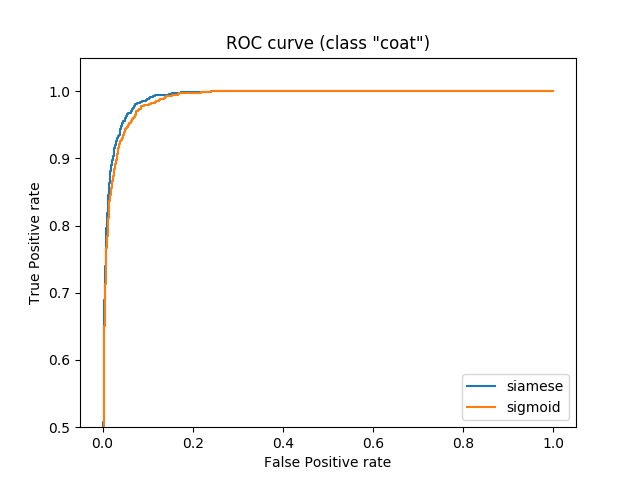
\includegraphics[scale=0.25]{fasion_roccurve.png}
        \end{minipage}
          \begin{minipage}{0.50\hsize}
            \centering
            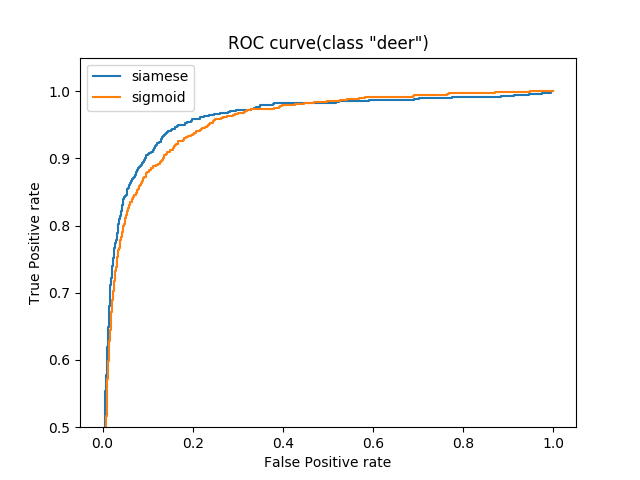
\includegraphics[scale=0.25]{roc_curve.png}
        \end{minipage}
\end{tabular}
\caption{ROC curve in binary classification}
\label{fig:roc-bi}
\end{figure}


\subsection{Multi-class Classification}



For baseline model, learning of end to end is performed by crossentropy loss of Equation (\ref{eq:multi crossentropy}) using softmax function as the activation function of $K$ output layers.
This is a general multi-class classifier model using a neural network. \par
Comparison experiments compare the AUC scores of these two models.
For each model, accuracy evaluation based on the prediction result $\hat{\bm t}_n$ of the model is also performed.
$\hat{\bm t}_n$ is a $K$-dimensional one-hot-vector with $\hat{t}_n^{(k)}$ as an element satisfying the following condition.
\begin{align} \label{eq:accuracy}
\hat{t}_n^{(k)}=\left\{
\begin{array}{cc}
1 & (k = argmax(y_n^{(0)}, y_n^{(1)}, \cdots, y_n^{(K)})) \\ 
0 & (otherwise)
\end{array}
\right.
\end{align} \par
As a result of comparative experiments, also in the case of multi-class, improvement of AUC score was seen.
And, siamese network exceeds the score in accuracy evaluation.
%By the way, in general crossentropy loss which uses sigmoid function as output activation function is used for binary classification using neural network.
%This sigmoid crossentropy considers positive and negative samples independently.
%On the other hand, the siamese network learns the metric between samples.






In the case of multi-class classification, each model is evaluated with accuracy and AUC.
We regard that each unit of the output layer of each model solves the binary classification problem classifying target class and other classes.
So, it is calculated AUC for each output unit.
The average score of each calculated AUC is evaluated as the AUC score in the case of multi-class. 
Likewise, ROC curves are drawn for each model and shown in the figure \ref{fig:roc-mul}. \par
The learning rate of MomentumSGD is initially set at 0.01,  and  divided  by  10  every  100 epochs.  
The  momentum parameter  is  fixed  to  0.9.  
The parameter $m$ of siamese network is fixed at 10.
In  addition,  for  each  model,  experiments  are conducted  with  five  kinds  of  initial  weight  values,  and  this average score is posted as a result. \par
The accuracy and AUC for each dataset are shown in Figure \ref{fig: multi auc and acc}.
%In  order  to  prevent  over  learning, regularization  term  is  added  to  loss  as  necessary.
\begin{figure}[ht]
\begin{center}
\scalebox{0.7}{
\begin{tabular}{|c|c|c||c|c|c|} \hline
ROC-AUC & baseline & siamese & accuracy &  baseline & siamese  \\ \hline \hline
fasionMNIST & $0.9932$    & ${\bf 0.9941}$  &  fasionMNIST  & $0.9040$   &  ${\bf 0.9163}$ \\ \hline
CIFAR10  & $0.9601$      &  ${\bf 0.9635}$     &  CIFAR10   & $0.7219$     &${\bf 0.7538}$ \\ \hline
\end{tabular}}
\end{center}
\caption{AUC and accuracy of multi classification}
\label{fig: multi auc and acc}
\end{figure} \par
As can be seen the figure, siamese network has higher accuracy and AUC score for both datasets.
Particularly in classification of CIFAR10, accuracy has improved by about 3$\%$. \par


\begin{figure}[ht]
\centering
\begin{tabular}{c}
        \begin{minipage}{0.50\hsize}
            \centering
            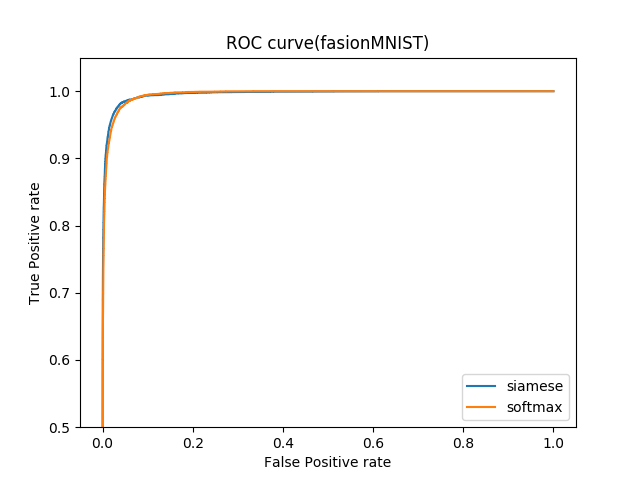
\includegraphics[scale=0.25]{fasion_multiroccurve.png}
        \end{minipage}
          \begin{minipage}{0.50\hsize}
            \centering
            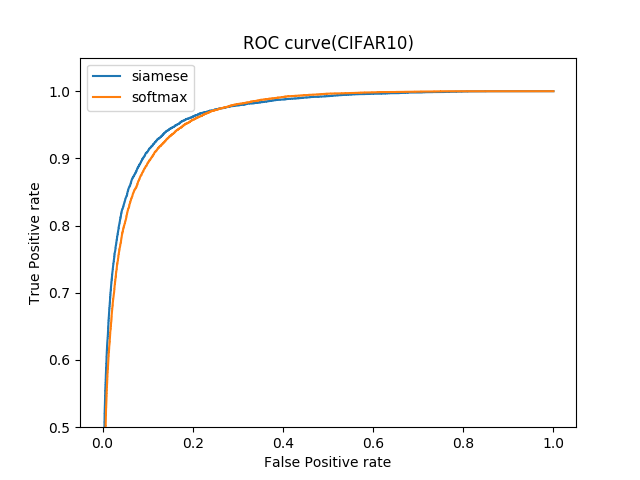
\includegraphics[scale=0.25]{multiroc_curve.png}
        \end{minipage}
\end{tabular}
\caption{ROC curve in multi-class classification}
\label{fig:roc-mul}
\end{figure}
For both data sets, we can see that the proposed model depicts a slightly larger ROC curve.
From the above, it can be seen that the feature vector of the siamese network contributes to increasing the ROC-AUC score.


\section{Conclusion and Future Works}
\thispagestyle{empty}

A series of experiments showed that in the binary classification, also Siamese Network has high performance on ROC-AUC optimization.
In many cases, it shows higher performance than baseline's classification model.
In addition, it can be confirmed that the logistic regression model that estimates the posterior probability from the output of Siamese Network also works effectively to optimize ROC-AUC.
It can also be extended to the multi class classification task, showing a higher score than the baseline model in both accuracy and ROC-AUC score.
The Siamese Network that conducts pairwise learning is extended to Triplet Network where learning are performed in triplets.
Elad Hoffer et al. \cite{triplet} proposed Triplet Network to input samples in triplets.
They extract feature vectors from triplicate samples and extract embedded representations for classification by clustering their feature vectors.
Then, the representation is converted to a posterior probability by a regression model, and class estimation is performed.
However, the results are inferior to conventional methods for many datasets.
Therefore, we need to verify how the result changes by extension of network based on binary classification like ours.

And in this paper, we performed two stages of learning to estimate posterior probability, but a model that learns up to posterior probability estimation with one model is also conceivable.
In future work, we will consider a model that simultaneously performs margin maximization between samples and posterior probability estimation.



\begin{thebibliography}{4}

\bibitem{Vapnik1963}
V.Vapnik,  and A. Lerner, ``A Pattern Recognition Using Generalized Portrait Method''  Automation and Remote Control, Vol.24, No.6, pp.774-780, 1963. 

\bibitem{SVM1995}
C. Cortes and V. Vapnik, 
``Support vector networks" 
Machine Learning, 20:273–297, 1995.

\bibitem{RankSVM}
R. Herbrich,  T. Graepel, and K. Obermayer, 
``Large margin rank boundaries for ordinal regression". 
In B. Smola and S. Schoelkopf (Eds.), Advances in large margin classifiers. Cambridge, MA: MIT Press, 2000.

\bibitem{ROCAUC}
O. Chapelle and S. S. Keerthi.  Efficient algorithms for ranking with SVMs. Information Retrieval, 13:201–215, June 2010.

\bibitem{Krizhevsky2012}
A. Krizhevsky, I. Sutskever, and G. E. Hinton,
``ImageNet classification with deep convolutional neural networks,''
Proc. Conf. Neural Information Processing Systems, pp.1097-1105, 2012.

\bibitem{Bromely1993}
J. Bromley, I. Guyon, Y. LeCun, E. S\"ackinger, and R. Shah, 
``Signature verification using a siamese time delay neural network,''
in {Advances in Neural Information Processing Systems}, Vol.6 (NIPS 1993), 1993.

\bibitem{Chopra2005}
S. Chopra,  R. Hadsell, and Y. LeCun,
``Learning a similarity metric discriminatively, with application to face verification,'' 
Proc. of the IEEE Computer Society Conference on Computer Vision and Pattern Recognition (CVPR2005), Vol. 1, pp. 539–546, 2005.

\bibitem{Hadsell2006}
R. Hadsell, S. Chopra, and Y. LeCun, 
``Dimensionality reduction by learning an invariant mapping,''
Proc. of 2006 IEEE computer society conference on Computer Vision and Pattern Recognition (CVPR2006), Vol. 2, pp. 1735–1742. 2006.

%\bibitem{Matusugu2003}
%M. Matusugu,  K. Mori, Y. Mitari, Y. Kaneda, ``Subject independent facial expression recognition with robust face detection using a convolutional neural network,'' Neural Networks. 16 (5): 555–559, 2003. 

\bibitem{He2016}
K. He, X. Zhang, S. Ren, and J. Sun, ``Deep Residual Learning for Image Recognition,'' Proc. of CVPR2016.

\bibitem{He2017}
K. He, G. Gkioxari, P. Dollár, R. Girshick, ``Mask R-CNN,'' Proc. of ICCV2017.

\bibitem{Ronneberger2015}
O. Ronneberger, P. Fischer, and T. Brox, ``U-Net: Convolutional Networks for Biomedical Image Segmentation,'' Proc. of Medical Image Computing and Computer-Assisted Intervention (MICCAI), Springer, LNCS, Vol.9351, pp.234--241, 2015.

\bibitem{triplet}
E. Hoffer, N. Ailon. 
"Deep Metric Learning Using Triplet Network",
In: Feragen A., Pelillo M., Loog M. (eds) Similarity-Based Pattern Recognition. Lecture Notes in Computer Science, vol 9370. Springer, Cham, 2015.
\end{thebibliography}


%\section*{Appendix: Springer-Author Discount}
%
%LNCS authors are entitled to a 33.3\% discount off all Springer
%publications. Before placing an order, the author should send an email, 
%giving full details of his or her Springer publication,
%to \url{orders-HD-individuals@springer.com} to obtain a so-called token. This token is a
%number, which must be entered when placing an order via the Internet, in
%order to obtain the discount.
%
%\begin{comment}
%\section{Checklist of Items to be Sent to Volume Editors}
%Here is a checklist of everything the volume editor requires from you:
%
%
%\begin{itemize}
%\settowidth{\leftmargin}{{\Large$\square$}}\advance\leftmargin\labelsep
%\itemsep8pt\relax
%\renewcommand\labelitemi{{\lower1.5pt\hbox{\Large$\square$}}}
%
%\item The final \LaTeX{} source files
%\item A final PDF file
%\item A copyright form, signed by one author on behalf of all of the
%authors of the paper.
%\item A readme giving the name and email address of the
%corresponding author.
%\end{itemize}
%
%\end{comment}

\thispagestyle{empty}
\end{document}

